% AgriNova --- NCSC Project Report
% Theme: Science and Innovation for Sustainability
% Group members: Shikha Sharma, Samriddhi Ghosh --- Class XI, KV Dum Dum
\documentclass[12pt,a4paper]{article}

\usepackage[a4paper,margin=2.2cm]{geometry}
\usepackage[T1]{fontenc}
\usepackage[utf8]{inputenc}
\usepackage{mathptmx}
\usepackage{amssymb}
\usepackage{microtype}
\usepackage{setspace}
\usepackage{xcolor}
\usepackage{graphicx}
\usepackage{tikz}
\usetikzlibrary{arrows.meta,positioning,calc,shapes.geometric,fit,decorations.pathreplacing}
\usepackage{pgfplots}
\pgfplotsset{compat=1.17}
\usepackage{booktabs}
\usepackage{tabularx}
\usepackage{array}
\usepackage{colortbl}
\usepackage{caption}
\usepackage{enumitem}
\usepackage{titlesec}
\usepackage{fancyhdr}
\usepackage{hyperref}

\hypersetup{
  colorlinks=true,
  linkcolor=nvgreen,
  urlcolor=nvgreen,
  citecolor=nvgreen,
  pdftitle={AgriNova --- NCSC Project Report},
  pdfauthor={Shikha Sharma, Samriddhi Ghosh}
}

\definecolor{nvgreen}{HTML}{1F4D3A}
\definecolor{nvleaf}{HTML}{3D6B54}
\definecolor{nvsaff}{HTML}{9A6B32}
\definecolor{nvink}{HTML}{1D1D1F}
\definecolor{nvmuted}{HTML}{6E6E73}
\definecolor{nvline}{HTML}{E6E4DF}
\definecolor{nvband}{HTML}{EEF3F0}
\definecolor{nvpaper}{HTML}{F7F6F2}

\pagestyle{fancy}
\fancyhf{}
\fancyhead[L]{\small\color{nvmuted}NCSC \textbullet\ Science and Innovation for Sustainability}
\fancyhead[R]{\small\color{nvmuted}AgriNova}
\fancyfoot[C]{\small\color{nvmuted}\thepage}
\renewcommand{\headrulewidth}{0.3pt}
\renewcommand{\footrulewidth}{0pt}

\titleformat{\section}{\large\bfseries\color{nvgreen}}{\thesection}{0.8em}{}
\titleformat{\subsection}{\normalsize\bfseries\color{nvleaf}}{\thesubsection}{0.7em}{}
\titleformat{\subsubsection}{\normalsize\bfseries\color{nvsaff}}{\thesubsubsection}{0.6em}{}
\titlespacing*{\section}{0pt}{1.15em}{0.45em}
\titlespacing*{\subsection}{0pt}{0.9em}{0.3em}

\setlist[itemize]{leftmargin=1.15em,itemsep=0.15em,topsep=0.25em}
\setlist[enumerate]{leftmargin=1.25em,itemsep=0.15em,topsep=0.25em}
\captionsetup{font=small,labelfont={bf,color=nvgreen},skip=4pt}

\setlength{\headheight}{15pt}
\onehalfspacing
\setlength{\parskip}{0.4em}
\setlength{\parindent}{0pt}
\newcommand{\tick}{$\square$\ }
\newenvironment{conv}[1]{%
  \par\vspace{0.55em}%
  {\small\bfseries\color{nvleaf}#1}\par\vspace{0.2em}%
  \noindent{\color{nvgreen}\vrule width 2.4pt}\hspace{0.65em}%
  \begin{minipage}[t]{\dimexpr\linewidth-1.0em\relax}\small
}{%
  \end{minipage}\par\vspace{0.25em}%
}

% ---------------------------------------------------------------------------
\begin{document}
\thispagestyle{empty}
\begin{tikzpicture}[remember picture,overlay]
  \fill[nvgreen] (current page.north west) rectangle ([yshift=-18mm]current page.north east);
  \fill[nvsaff] (current page.north west) ++(0,-18mm) rectangle ++(\paperwidth,1.6mm);
\end{tikzpicture}

\vspace*{6mm}
\begin{center}
{\color{nvgreen}\small NATIONAL CHILDREN'S SCIENCE CONGRESS}\\[0.35em]
{\color{nvmuted}\footnotesize Theme: \textit{Science and Innovation for Sustainability}}\\
{\color{nvmuted}\footnotesize Sub-themes: Waste Management \textbullet\ Food, Agriculture \& Health}\\[1.1em]
{\LARGE\bfseries\color{nvgreen} AGRINOVA}\\[0.35em]
{\large\color{nvink} Turning crop residue into income --- not smoke, not drain waste}\\[0.55em]
{\small\itshape\color{nvmuted} Predict.\ Protect.\ Prosper.\ Recycle.}\\[1.15em]
\begin{tabular}{@{}ll@{}}
\textbf{Group members} & Shikha Sharma \textbullet\ Samriddhi Ghosh\\
\textbf{Class} & XI (upper age group)\\
\textbf{School} & Kendriya Vidyalaya Dum Dum, Kolkata\\
\textbf{Language} & English\\
\textbf{Field area} & Madhyamgram \& Barasat (nearby) \textbullet\ Punjab by phone\\
\textbf{Guide teacher} & \rule{5.4cm}{0.4pt}\\
\end{tabular}
\end{center}

\vspace{0.7em}
{\color{nvgreen}\rule{\textwidth}{0.6pt}}

\section*{Abstract}

AgriNova asks a local, measurable question: why does rice straw still leave the farm as smoke in Punjab and as mixed drain waste in West Bengal, when biomass plants, paper mills and compost pads already buy the same material? The missing step is a listing --- quantity, moisture, neighbourhood --- that a small farm and a nearby gate can both see. This project names that step and tests AgriNova as the abatement tool.

Work had two parts. Part~I mapped rice straw from published CRM, SWM and air-quality notes. Part~II is the Class~XI field book from Kendriya Vidyalaya Dum Dum. Ten farmers were closed in September~2025: six at the door in Madhyamgram and Barasat, starting at Hridaypur, and four in Punjab by phone with family contacts, plus two plant-floor calls and two local civic officers (Councillor, Ward~21, Barasat Municipality; Sanitary Inspector, Madhyamgram Municipality). AgriNova at \url{https://agrinova-ochre.vercel.app} was then used as a demonstration desk on those sheets.

Last season, three of four Punjab phone sheets were burns; five of six local Bengal sheets were dump, mix or stack; only two of ten sold. Eight would list if a trolley came in five days. Officers see mixed drain waste and conservancy complaints, not tonnes utilised. The live desk matched a Kharar burn example and a Doltala dump example to moisture-aware gates.

The gap is not another scheme pamphlet. It is a shared listing with moisture, buyer and pickup time. On this 10-farm book, about 72~t would move if the eight ``yes'' lots listed --- a cluster demonstration, not a state forecast. Carbon figures are estimates, not certified credits.

\vspace{0.15em}
{\footnotesize\textit{Name \& address of Guide Teacher:} \rule{9.4cm}{0.4pt}}

\section*{Why this project?}
Burned or dumped straw is wasted biomass, dirty air, and zero farm cash. Punjab's short sowing window and Bengal's wet leftover fail at one point: the farmer has no plant number and the plant has no small lot. From Kendriya Vidyalaya Dum Dum we can walk that gap in Madhyamgram and Barasat, and hear the burn clock by phone. AgriNova is the listing this study now tests.

\tableofcontents
\newpage

% ===========================================================================
\section*{Part I --- Selection of the problem and basic information}
\addcontentsline{toc}{section}{Part I --- Selection of the problem and basic information}

\section{Selection of the problem}
The focal theme asks for science that makes a local waste stream less harmful. We are Class~XI students at Kendriya Vidyalaya Dum Dum. The stream we can actually walk to is peri-urban paddy leftover in \textbf{Madhyamgram and Barasat} (North 24 Parganas): straw stacked wet, pushed into a drain, or mixed into municipal biodegradable waste. These neighbourhoods sit inside the Kolkata Metropolitan area, so farm leftover and city conservancy meet on the same lane. Punjab enters as a \textbf{phone comparison} --- four family-contact sheets --- because that is the published burn belt, and one listing has to work on both clocks.

The visible problem is not ``farmers are careless.'' It is a clock. In Punjab, paddy comes off and wheat must go in within about ten to fifteen days. Burning is the two-hour option. In West Bengal the clock is wetter: straw sits, rots, is pushed into a canal, or is mixed into household waste that the municipality then has to lift as mixed biodegradable matter. Compost plants a few kilometres away still report hungry pads.

We selected this problem because (i)~the material is the same --- rice straw; (ii)~Madhyamgram--Barasat fails by dump/mix, Punjab-by-phone fails by burn, so one desk must serve both; (iii)~a municipal compost pad already exists while drains still take mixed straw; (iv)~two Class~XI students can finish ten named sheets nearby and by phone, then demonstrate AgriNova, without claiming a census.

\subsection{Hypothesis}
If a smallholder can list last season's straw with a moisture note and is promised pickup inside five days, then selling (or gifting to a plant) will replace burning or dumping as the default, provided the net gate price after freight is positive.

\subsection{Objectives}
\begin{enumerate}[leftmargin=1.4em]
  \item Record what happened to most of last season's residue among a small, named field pack.
  \item Name the main barrier between the field and the plant gate.
  \item Check whether plant-floor staff will take two-to-six acre lots if moisture is declared.
  \item Check what junior officials currently put in the register.
  \item Field-test AgriNova on the same clusters and propose an abatement system.
\end{enumerate}

\subsection{Need and relevance}
Madhyamgram and Barasat are not a remote paddy belt. They are peri-urban North 24 Parganas, next to our school. Conservancy already lifts mixed biodegradable waste under SWM Rules, 2016, while small leftover piles never become a lot. Punjab's published burn window is the comparison clock we could only hear by phone. The need is a listing that both clocks can use --- Bangla at the door, Punjabi on the call --- without putting farmer numbers on a municipal screen.

\section{Basic information about the element chosen}
The element is \textbf{rice straw} (paddy residue), sometimes mixed with wheat stubble or jute leftover.

\begin{itemize}
  \item \textbf{How much grows on a small farm.} Published residue-to-grain work used by IARI / PAU puts straw in a band of about 1.8--2.4~tonnes per acre of paddy. This project used 2.0~t/acre as a conservative working figure when a farmer could not weigh a pile.
  \item \textbf{What it is chemically useful for.} Dry straw is lignocellulose. Biomass plants burn it under spec; paper mills want furnish below a moisture cap; compost and biomethanation pads want a clean biodegradable lot, not mixed drain waste.
  \item \textbf{What burning does.} Open burning returns almost no cash to the farm, strips surface organic matter, and loads the winter airshed with particulates. Literature used as context (not as our sensor) puts peak post-harvest contribution of residue fire to Delhi--NCR PM$_{2.5}$ in a 30--40\% band on some episode days.
  \item \textbf{What dumping does.} Straw that never becomes a lot becomes a municipal problem. Solid Waste Management Rules, 2016, already ask urban local bodies to process biodegradable waste. Farm straw that enters the drain as mixed wet waste is the wrong specification for those plants.
\end{itemize}

Table~\ref{tab:element} is the working sheet we carried --- not a laboratory assay.

\begin{table}[h]
\centering
\caption{Data elements defined before the survey (what we would actually ask).}
\label{tab:element}
\small
\begin{tabularx}{\textwidth}{@{}lXl@{}}
\toprule
\textbf{Element} & \textbf{Why it matters} & \textbf{How recorded} \\
\midrule
Residue fate & Burn / dump / sell / mix & One choice \\
Harvest--sow window & Clock that makes burning rational & Four bands \\
Own buyer phone & Matching gap & Yes / broker / no \\
Main barrier & Cause, not slogan & One choice \\
5-day pickup & Product test & Yes / maybe / no \\
Plant moisture spec & Gate argument & Buyer choice \\
Register contents & What government already sees & Official choice \\
\bottomrule
\end{tabularx}
\end{table}

\section{Previous studies (defining the problem)}
We did not invent stubble burning or eastern residue waste. We used a short, cited shelf so the problem is defined before our 10 sheets.

\textbf{Policy.} The National Policy for Management of Crop Residue (NPMCR, 2014) asks states to map surplus and move it in-situ or to industry. The Crop Residue Management (CRM) machinery push --- Happy Seeders, balers, custom-hiring --- was densest in the north-west burn belt. Solid Waste Management Rules, 2016 (MoEFCC) require segregation and processing of biodegradable waste, including agricultural leftover that enters the urban stream. NGT orders on residue fire set fines and action plans; they do not themselves create a buyer phone in the village.

\textbf{Air and volume.} SAFAR / IITM and CPCB episode notes are the public source for the 30--40\% PM$_{2.5}$ band on peak days. MoEFCC and Punjab CRM notes round paddy straw in Punjab to the order of 15--20 million tonnes a kharif, a large share of which is still burned in a short window. These numbers are context. They are not our sample.

\textbf{Farm economics.} Commission for Agricultural Costs and Prices MSP cards (common paddy about Rs~2300/q in the 2024--25 marketing season we used) explain why the grain is sold and the straw is treated as a nuisance. Biomass tender ranges quoted in CRM write-ups sit roughly Rs~600--1200/t at the gate; transport and broker cuts decide whether a two-acre farm bothers. A 3-acre Doltala pile at 2.0~t/acre is about 6~t. At Rs~700/t that is about Rs~4,200 before freight --- enough to notice, not enough to hire a broker for one house.

\textbf{Local processing.} SWM Rules already require urban local bodies to process biodegradable waste. Madhyamgram and Barasat sit inside that urban stream: a conservancy pad can take a clean lot, but mixed drain straw is the wrong specification. The published shelf tells us the pad exists. It does not tell us whether a 1.5-acre heap in Hridaypur ever becomes a lot.

\textbf{What the shelf does not give.} NPMCR maps residue. SWM Rules map urban processing. Neither builds a place where a 3-acre farmer in Doltala, a conservancy pad, and a ward councillor share one lot without putting KCC numbers on a portal. That absence is the problem we measured.

\section{Analysis of the problem and measurement}
The problem has three clocks, not one.

\begin{enumerate}
  \item \textbf{Farmer clock.} Ten to fifteen dry days in Punjab; longer but wetter days in Bengal. Burning or dumping is the option that fits the clock.
  \item \textbf{Plant clock.} A biomass or paper unit needs hundreds of tonnes in a fortnight, at a moisture cap (about 15\% in the Punjab plants we asked; 16--18\% in the Bengal compost/paper gates). A two-acre pile is invisible unless someone aggregates it.
  \item \textbf{Officer clock.} Ward conservancy and the sanitary inspector file mixed-waste complaints. The register does not answer ``how many tonnes left this ward as a specified lot?''
\end{enumerate}

Measurement, for this project, is therefore not a satellite burn count. It is a small KAP (knowledge--attitude--practice) pack plus one operational test: can a listing with moisture find a plant that will lift it?

Figure~\ref{fig:problem} is the causal sketch we used before writing the sheet.

\begin{figure}[h]
\centering
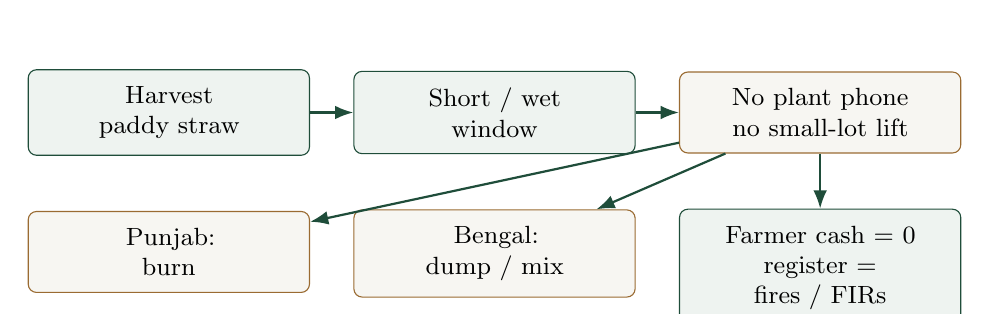
\begin{tikzpicture}[
  font=\small,
  box/.style={draw=nvgreen, rounded corners=3pt, align=center, inner sep=6pt, fill=nvband, text width=3.15cm},
  bad/.style={draw=nvsaff, rounded corners=3pt, align=center, inner sep=6pt, fill=nvpaper, text width=3.15cm},
  arr/.style={-{Latex}, thick, nvgreen}
]
\node[box] (h) {Harvest\\paddy straw};
\node[box, right=0.55cm of h] (w) {Short / wet\\window};
\node[bad, right=0.55cm of w] (n) {No plant phone\\no small-lot lift};
\node[bad, below=0.7cm of h] (b) {Punjab:\\burn};
\node[bad, below=0.7cm of w] (d) {Bengal:\\dump / mix};
\node[box, below=0.7cm of n] (z) {Farmer cash = 0\\register = fires / FIRs};
\draw[arr] (h) -- (w);
\draw[arr] (w) -- (n);
\draw[arr] (n) -- (b);
\draw[arr] (n) -- (d);
\draw[arr] (n) -- (z);
\end{tikzpicture}
\caption{Problem sketch used to design the questionnaire. The missing object is the middle box --- not a new law.}
\label{fig:problem}
\end{figure}

\subsection{Suggested solutions (before field testing)}
Four options sat on the table. We kept only what a school team could test.

\begin{enumerate}
  \item \textbf{More machines only.} Happy Seeder and balers exist in Punjab CRM notes. Madhyamgram--Barasat households we asked do not have a shared baler slot they can book. Machines without a list of lots still arrive late.
  \item \textbf{Fines only.} Fines change the cost of burning; they do not create a gate price or a trolley, and they do not stop drain dumping here.
  \item \textbf{Scheme PDF / helpline.} Local sheets asked for Bangla voice and a pickup slot, not another pamphlet.
  \item \textbf{Matching desk (chosen).} One listing: quantity, moisture, neighbourhood. One score: distance, demand, moisture fit. One pickup slot. Ward / SI sees tonnes utilised versus dumped --- no farmer phone on the officer screen.
\end{enumerate}

That fourth option is AgriNova. Part~II tests whether the people who would use it --- small farmers, plant clerks, junior officials --- describe the same gap.

% ===========================================================================
\newpage
\section*{Part II --- Field testing of the solution}
\addcontentsline{toc}{section}{Part II --- Field testing of the solution}

\section{Description: survey --- area, duration, method}
Six Bengal sheets were taken at the door, at the chaupal, or on a short local call in Madhyamgram and Barasat. Four Punjab sheets were taken by phone through family contacts. Two plant-floor talks were phone-only. Two civic officers are people a Dum Dum student can actually reach: the Ward~21 councillor of Barasat Municipality, and the sanitary inspector of Madhyamgram Municipality.

Shikha kept the Bangla / Hindi local sheets and the Barasat ward conversation. Samriddhi kept the Madhyamgram conservancy conversation and entered ticks the same evening. Punjab calls were shared: one student asked, the other wrote. Each farmer sitting lasted 12--18 minutes. Options were read aloud. The last line was taken in the speaker's words.

What we saw locally, before the ticks: in Doltala, Hridaypur and on the Ward~21 edge, leftover straw sat in a wet heap or had already been mixed into household waste that the municipality lifts as mixed biodegradable matter. Nobody we asked had a compost-pad number on their phone. That observation set the sheet --- fate, own plant phone, five-day pickup --- before we wrote a line of software.

\textbf{Duration.} Local visits in \textbf{September 2025}, starting at Hridaypur (Tapas Mondal) and then Doltala, Noapara, Michael Nagar, Nabapally and the Ward~21 neighbourhood. Punjab comparison calls were made the same month, about last season's straw. Residue on the Madhyamgram--Barasat lane was already sitting from the previous crop after the monsoon; this is not an October--November harvest-window study.

\textbf{Rules.} (i)~1.5--8 acre farms --- the size a mill skips; (ii)~stop at ten farmer sheets (6 local + 4 phone); (iii)~no secretariat, no DC, no managing director; (iv)~no Aadhaar, KCC or mobile stored.

\textbf{Local area (6).} Madhyamgram outgrowth (Doltala, Noapara, Michael Nagar) and Barasat (Hridaypur, Nabapally, Ward~21 neighbourhood). North 24 Parganas. Walkable or a short auto from Dum Dum along Jessore Road / BT Road.

\textbf{Punjab by phone (4).} Kharar, Nabha, Ghanaur, Rajpura rural (Patiala belt). Call only. Used to test whether the same sheet still sees a burn clock.

\textbf{Closed count.} 10 farmers + 2 buyers (phone) + 2 officials = 14 sheets.

\begin{table}[h]
\centering
\caption{Field log (September 2025).}
\label{tab:log}
\small
\begin{tabularx}{\textwidth}{@{}>{\raggedright\arraybackslash}p{3.2cm}>{\raggedright\arraybackslash}X>{\raggedright\arraybackslash}X@{}}
\toprule
\rowcolor{nvband}
When & Where & Who \\
\midrule
Early September & Hridaypur, Barasat & Tapas Mondal (doorstep) \\
Same week & Doltala; Noapara; Michael Nagar & Ramesh Das, Anil Ghosh, Kamal Haldar \\
Mid September & Ward 21 neighbourhood; Nabapally & Sukumar Roy, Arun Bhattacharya \\
Mid September & Barasat Municipality / phone & Dr.\ Bibartan Saha (Ward 21) \\
Mid September & Madhyamgram conservancy & Sudip Biswas (SI); Biswajit Ghosh (pad) \\
Late September & Phone (Patiala belt) & Jaswinder, Harpreet, Balwinder, Gurmeet; Rakesh Kumar \\
\bottomrule
\end{tabularx}
\end{table}

\section{Questionnaire used / data collected}
Three short instruments. A long schedule was refused at the first Madhyamgram sitting. Options were read aloud. One sentence was taken in the speaker's words. Mode --- doorstep or phone --- was marked on every farmer sheet.

\subsection{Farmer sheet (10 closed)}
\begin{enumerate}[leftmargin=1.5em]
  \item What happened to \emph{most} of last season's straw? \tick{} Sold / gifted \quad \tick{} Stacked, dumped or left to rot \quad \tick{} Burned on a dry window \quad \tick{} Mixed into household / municipal waste
  \item Harvest to next sowing --- how many days? \tick{} Under 10 \quad \tick{} 10--15 \quad \tick{} 16--25 \quad \tick{} More than 25
  \item Do you have a plant's own phone number? \tick{} Yes, own \quad \tick{} Only a broker \quad \tick{} None
  \item If you did not sell, what was the main barrier? \tick{} No buyer phone \quad \tick{} Straw too wet \quad \tick{} Transport eats the gate price \quad \tick{} Did not know a pad/mill exists \quad \tick{} I did sell
  \item If a trolley came in five days, would you list this lot? \tick{} Yes \quad \tick{} Maybe \quad \tick{} No
  \item Language you want the listing in? \tick{} Bangla / Bangla voice \quad \tick{} Punjabi \quad \tick{} Hindi \quad \tick{} English
  \item One sentence, in your words, about last season's straw.
\end{enumerate}

\subsection{Buyer sheet (2, phone)}
\begin{enumerate}[leftmargin=1.5em]
  \item Plant type and gate (compost pad / biomass / paper).
  \item Moisture you will lift, and whether mixed drain straw is refused.
  \item Do 2--6 acre lots reach this gate without a broker?
  \item Would a listing with moisture help you send one trolley?
  \item One sentence from the cabin / pad.
\end{enumerate}

\subsection{Official sheet (2)}
Post as printed on the municipality board only: Councillor, Ward~21, Barasat; or Sanitary Inspector, Madhyamgram.
\begin{enumerate}[leftmargin=1.5em]
  \item What goes into the register today?
  \item Biggest gap you see between farm leftover and the pad?
  \item Would an aggregate view of tonnes utilised --- without farmer phones --- help the weekly note?
  \item One sentence. Notes of a student conversation, not a ULB circular.
\end{enumerate}

\section{Activities taken up}
\begin{enumerate}
  \item September field start at Hridaypur (Tapas Mondal), then five more local sheets.
  \item Closed 10 farmer sheets (6 nearby, 4 phone) and 2 civic conversations.
  \item Two plant-floor phone calls --- Madhyamgram conservancy pad and a Punjab biomass cabin (family contact).
  \item Built AgriNova: \url{https://agrinova-ochre.vercel.app}.
  \item Demonstration walk-through on that desk using this book (Ramesh Das dump lot; Jaswinder Singh burn lot) plus the in-app Punjab case-study cluster as a labelled example.
\end{enumerate}

Figure~\ref{fig:system} is the desk we tested.

\begin{figure}[h]
\centering
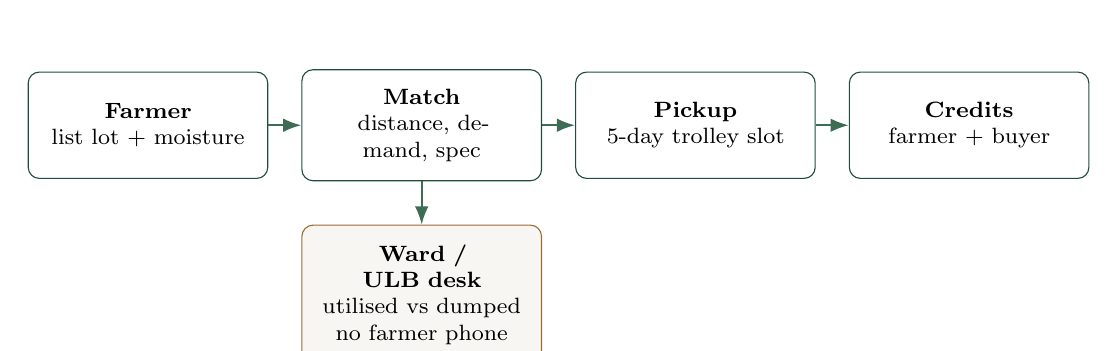
\begin{tikzpicture}[
  font=\footnotesize,
  d/.style={draw=nvgreen, rounded corners=4pt, align=center, inner sep=7pt, fill=white, text width=2.55cm, minimum height=1.35cm},
  g/.style={draw=nvsaff, rounded corners=4pt, align=center, inner sep=7pt, fill=nvpaper, text width=2.55cm, minimum height=1.35cm},
  arr/.style={-{Latex}, thick, nvleaf}
]
\node[d] (f) {\textbf{Farmer}\\list lot + moisture};
\node[d, right=0.42cm of f] (m) {\textbf{Match}\\distance, demand, spec};
\node[d, right=0.42cm of m] (p) {\textbf{Pickup}\\5-day trolley slot};
\node[d, right=0.42cm of p] (c) {\textbf{Credits}\\farmer + buyer};
\node[g, below=0.55cm of m] (o) {\textbf{Ward / ULB desk}\\utilised vs dumped\\no farmer phone};
\draw[arr] (f) -- (m);
\draw[arr] (m) -- (p);
\draw[arr] (p) -- (c);
\draw[arr] (m) -- (o);
\end{tikzpicture}
\caption{AgriNova loop. Local officers see aggregates, not the farmer's number.}
\label{fig:system}
\end{figure}

\section{Analysis of data}
\subsection{Farmers (n = 10)}
Table~\ref{tab:roster} is the whole book. Table~\ref{tab:fate} and Figure~\ref{fig:fate} add it up. Phone-Punjab is a burn pocket. Madhyamgram--Barasat is a dump-and-mix pocket. Only Balwinder (phone) and Anil (Noapara) sold last season.

\begin{table}[h]
\centering
\caption{Farmer book (n=10). Mode: D~doorstep/nearby, P~phone. Fate: B~burn, K~stack/dump, S~sold, M~mixed waste.}
\label{tab:roster}
\scriptsize
\begin{tabularx}{\textwidth}{@{}>{\raggedright\arraybackslash}X>{\raggedright\arraybackslash}Xccrccc@{}}
\toprule
\rowcolor{nvband}
Name & Place & How & St & Ac & Fate & Phone & 5d \\
\midrule
Ramesh Das & Doltala, Madhyamgram & D & WB & 3.0 & K & none & Y \\
Sukumar Roy & Ward 21, Barasat & D & WB & 2.0 & M & none & Y \\
Anil Ghosh & Noapara, Madhyamgram & D & WB & 4.0 & S & broker & Y \\
Tapas Mondal & Hridaypur, Barasat & D & WB & 1.5 & K & none & M \\
Kamal Haldar & Michael Nagar & D & WB & 3.5 & M & none & Y \\
Arun Bhattacharya & Nabapally, Barasat & D & WB & 5.0 & K & none & Y \\
Jaswinder Singh & Kharar (phone) & P & PB & 6.0 & B & broker & Y \\
Harpreet Kaur & Nabha (phone) & P & PB & 4.5 & B & none & Y \\
Balwinder Singh & Ghanaur (phone) & P & PB & 8.0 & S & own & Y \\
Gurmeet Singh & Rajpura rural (phone) & P & PB & 3.0 & B & none & M \\
\bottomrule
\end{tabularx}
\end{table}

\begin{table}[h]
\centering
\caption{Last-season residue fate (this book only).}
\label{tab:fate}
\small
\begin{tabularx}{\textwidth}{@{}>{\raggedright\arraybackslash}Xcccc@{}}
\toprule
\rowcolor{nvband}
Fate & PB phone & Local WB & All & Share \\
\midrule
Burned on a dry window & 3 & 0 & 3 & 30\% \\
Stacked / left to rot or dump & 0 & 3 & 3 & 30\% \\
Sold / gifted & 1 & 1 & 2 & 20\% \\
Mixed into municipal waste & 0 & 2 & 2 & 20\% \\
\bottomrule
\end{tabularx}
\end{table}

\begin{figure}[h]
\centering
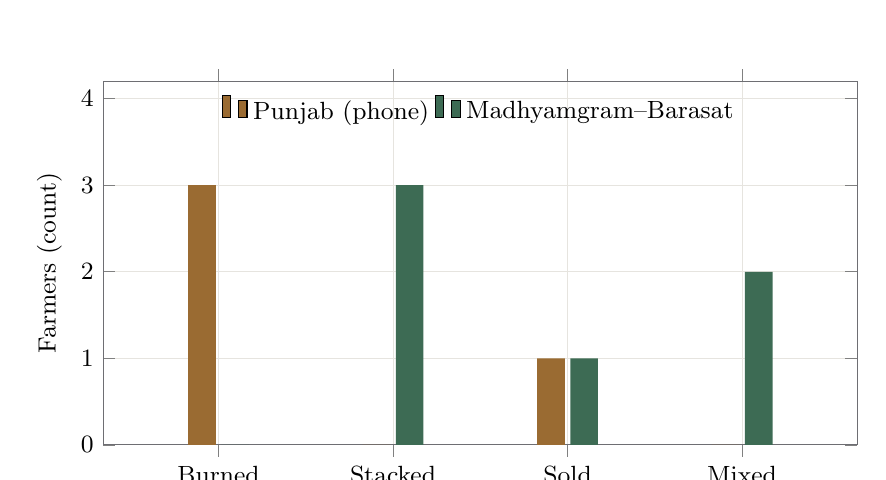
\begin{tikzpicture}
\begin{axis}[
  ybar,
  bar width=10pt,
  width=0.92\textwidth,
  height=6.2cm,
  ymin=0, ymax=4.2,
  ylabel={Farmers (count)},
  symbolic x coords={Burned,Stacked,Sold,Mixed},
  xtick=data,
  xticklabel style={font=\small},
  ylabel style={font=\small},
  tick label style={font=\small},
  legend style={font=\small, at={(0.5,0.98)}, anchor=north, legend columns=2, draw=none, fill=none},
  enlarge x limits=0.22,
  grid=major,
  major grid style={nvline},
  axis line style={nvmuted},
  ytick={0,1,2,3,4},
]
\addplot[fill=nvsaff, draw=none] coordinates {(Burned,3) (Stacked,0) (Sold,1) (Mixed,0)};
\addplot[fill=nvleaf, draw=none] coordinates {(Burned,0) (Stacked,3) (Sold,1) (Mixed,2)};
\legend{Punjab (phone), Madhyamgram--Barasat}
\end{axis}
\end{tikzpicture}
\caption{Same straw, two failure modes on ten named sheets.}
\label{fig:fate}
\end{figure}

\textbf{Window.} All four Punjab calls: under 10 or 10--15 days. Five of six local sheets: 16--25 days or more --- wet stall, not a dry sprint.

\textbf{Phone.} Own plant number: Balwinder only. Broker: Anil and Jaswinder. None: 7 of 10. The matching gap is seven households with nobody to call.

\textbf{Barrier} (did not sell): no buyer phone --- 5; straw too wet --- 2; transport --- 1; did sell --- 2.

\textbf{Language.} Bangla or Bangla-voice: 5 of the 6 local sheets. Punjabi: 3 of 4 calls. English: 0.

\textbf{Product test.} 8~Yes, 2~Maybe (Tapas, 1.5~ac, Hridaypur, still wet in September; Gurmeet, 3~ac, mill skips him). 0~No.

Reading the ten sheets together: Bengal fails after the monsoon, when a leftover heap is already wet and the municipality treats it as mixed biodegradable waste. Punjab-by-phone fails on a dry twelve-day clock, when burning is faster than waiting for a rumour of a trolley. The shared hole is the same: seven farms had no plant number; only Balwinder had his own. Anil sold once and still wants the moisture slip written before the truck leaves Noapara --- so even the ``sold'' row is a matching problem, not a success story we can copy.

\subsection{Conversations (as spoken)}
We wrote these the same evening, in English, from Bangla, Hindi or Punjabi. They are not polished speeches. The first sitting was Tapas Mondal at Hridaypur in early September.

\begin{conv}{Tapas Mondal --- Hridaypur, Barasat \textbullet\ doorstep, early September 2025 \textbullet\ 1.5~ac, stacked, Maybe}
We: What happened to last season's straw?\\
Tapas: You see that heap? Rain last week. Still wet inside. Who will bale 1.5 acres?\\
We: If a trolley came in five days?\\
Tapas: If four houses on this lane list together, a trolley might come. Alone, nobody comes. That is why I said maybe.
\end{conv}

\begin{conv}{Ramesh Das --- Doltala, Madhyamgram \textbullet\ doorstep \textbullet\ 3~ac, stacked, Yes}
We: Do you have a mill or pad number?\\
Ramesh: Straw sits by the drain. I asked a neighbour if any mill number is going around. Nobody has it.\\
We: If someone takes it as a lot?\\
Ramesh: Then I will not dump it. Give me a date. I will stack it clean.
\end{conv}

\begin{conv}{Sukumar Roy --- Ward~21 edge, Barasat \textbullet\ doorstep \textbullet\ 2~ac, mixed waste, Yes}
We: Where does the leftover go after rain?\\
Sukumar: We push it to the drain. Conservancy shouts, then they lift mixed waste anyway.\\
We: Would you send it to a pad if it took it clean?\\
Sukumar: Tell me a pad that will take it clean. I will send it. Speak in Bangla. I do not read a scheme PDF.
\end{conv}

\begin{conv}{Anil Ghosh --- Noapara, Madhyamgram \textbullet\ doorstep \textbullet\ 4~ac, sold once, Yes}
We: You sold last season. How?\\
Anil: Through a broker. Moisture fight at the gate. They cut the rate after the truck arrived.\\
We: Would you list again?\\
Anil: If the slip is made before the truck leaves Noapara, I will list again. Not after they wet-test at their gate and argue.
\end{conv}

\begin{conv}{Kamal Haldar --- Michael Nagar \textbullet\ doorstep \textbullet\ 3.5~ac, mixed, Yes}
We: Mixed into household waste?\\
Kamal: After two rains the heap smells. Conservancy already lifts mixed biodegradable from this lane. Straw goes with it.\\
We: Five-day pickup?\\
Kamal: If they come before it mixes, yes. After it mixes, what will they take?
\end{conv}

\begin{conv}{Arun Bhattacharya --- Nabapally, Barasat \textbullet\ doorstep \textbullet\ 5~ac, stacked, Yes}
We: Why is it still sitting?\\
Arun: Scheme PDF I cannot use. Nobody came. The pile is too wet for a mill rumour I heard last year.\\
We: Bangla listing?\\
Arun: Speak in Bangla. I will list. Five days is enough if the trolley is real.
\end{conv}

\begin{conv}{Jaswinder Singh --- Kharar \textbullet\ phone, late September \textbullet\ 6~ac, burned, Yes}
We: Last kharif --- what did you do with the straw?\\
Jaswinder: Twelve days for wheat. Last year I burned. WhatsApp rumours of a trolley come late.\\
We: If the date is on a listing you can see?\\
Jaswinder: If a trolley is on a date I can see, I will not light it. Punjabi. Not English PDF.
\end{conv}

\begin{conv}{Harpreet Kaur --- Nabha \textbullet\ phone \textbullet\ 4.5~ac, burned, Yes}
We: Same window as Kharar?\\
Harpreet: Ten to twelve days. No plant number in the house. Brother burned last year; we did the same.\\
We: Five-day pickup?\\
Harpreet: Yes, if it is before wheat sowing. After that the field is gone.
\end{conv}

\begin{conv}{Balwinder Singh --- Ghanaur \textbullet\ phone \textbullet\ 8~ac, sold, Yes}
We: You sold. Own number?\\
Balwinder: Yes, a biomass cabin. I am the largest of the four calls. The mill takes me because I can fill a trolley.\\
We: Would a listing still help?\\
Balwinder: For moisture, yes. Last year they cut me on wet bales. Put moisture on the slip before I load.
\end{conv}

\begin{conv}{Gurmeet Singh --- Rajpura rural \textbullet\ phone \textbullet\ 3~ac, burned, Maybe}
We: Why burn if a mill is in Rajpura?\\
Gurmeet: Mill skips 3 acres. Broker wanted a cut I would not pay. Easier to burn in the window.\\
We: Five-day pickup?\\
Gurmeet: Maybe --- if they pool me with a neighbour. Alone, they will skip me again.
\end{conv}

\begin{conv}{Biswajit Ghosh --- Madhyamgram conservancy pad \textbullet\ phone}
We: Will you lift 2--6 acre lots?\\
Biswajit: We are short of clean feedstock. Mixed drain straw we will not take.\\
We: Moisture on a listing?\\
Biswajit: If moisture is on a listing, I can send one trolley. Without it I am guessing, and I will not guess.
\end{conv}

\begin{conv}{Rakesh Kumar --- biomass cabin, Rajpura \textbullet\ phone (family contact)}
We: Small lots?\\
Rakesh: Rarely. We need bales and $\le$15\%. A loose wet heap from 3 acres does not enter this cabin.\\
We: Listing?\\
Rakesh: Only if it is baled and the moisture is written. Otherwise the gate argument starts.
\end{conv}

\begin{conv}{Dr.\ Bibartan Saha --- Councillor, Ward No.~21, Barasat Municipality \textbullet\ notes of a student conversation}
We: What is in the ward note today?\\
Dr.\ Saha: Complaints are drain and mixed waste. I do not see tonnes that left the ward as a lot.\\
We: A ward total without farmer phones?\\
Dr.\ Saha: That would help the weekly note. Keep names off the officer screen.
\end{conv}

\begin{conv}{Sudip Biswas --- Sanitary Inspector, Madhyamgram Municipality \textbullet\ notes of a student conversation}
We: What do you see on the conservancy round?\\
SI: Mixed biodegradable lift. Farm straw is not a specified lot.\\
We: If a desk stays at ULB level?\\
SI: Yes --- utilised versus dumped. No KCC on a portal. I will not put farmer mobiles on a municipal screen.
\end{conv}

\subsection{Buyers (n = 2, phone)}
\begin{table}[h]
\centering
\caption{Plant-floor phone talks. Rajpura cabin was a family-contact call.}
\label{tab:buyers}
\small
\begin{tabularx}{\textwidth}{@{}>{\raggedright\arraybackslash}p{2.6cm}>{\raggedright\arraybackslash}p{2.2cm}>{\raggedright\arraybackslash}p{3.4cm}>{\raggedright\arraybackslash}p{2.2cm}X@{}}
\toprule
\rowcolor{nvband}
Name & Post & Gate & Spec & Small lots / listing \\
\midrule
Biswajit Ghosh & Pad staff & Madhyamgram conservancy compost yard & $\le$18\%; no mixed drain waste & Almost never without a broker. Listing: yes. \\
Rakesh Kumar & Shift supervisor & Biomass cabin, Rajpura (phone) & $\le$15\% & Rarely. Listing: only if baled. \\
\bottomrule
\end{tabularx}
\end{table}

The local pad is hungry. The two-acre farm never calls. Mixed wet straw is refused. Rakesh will take a bale at $\le$15\%; he will not take Gurmeet's loose 3-acre heap. That split is enough to design a listing: compost-first for wet Madhyamgram--Barasat lots, biomass-first for dry Punjab phone lots.

\subsection{Government (n = 2)}
Both names are on the municipality boards. We asked for time; this is not an official ULB study.

\begin{table}[h]
\centering
\caption{Civic officers students could reach from Dum Dum.}
\label{tab:gov}
\small
\begin{tabularx}{\textwidth}{@{}>{\raggedright\arraybackslash}p{4.1cm}>{\raggedright\arraybackslash}p{3.3cm}X@{}}
\toprule
\rowcolor{nvband}
Name and post & Register today & Gap / desk \\
\midrule
Dr.\ Bibartan Saha, Councillor, Ward No.~21, Barasat Municipality & Ward complaints; mixed drain and conservancy calls & Compost pad sits hungry while farm leftover enters the drain as mixed waste. A ward view of tonnes utilised --- without farmer phones --- would help the weekly note. \\
Sudip Biswas, Sanitary Inspector, Madhyamgram Municipality & Conservancy / SWM complaints; mixed biodegradable lift & Farm straw is not a specified lot. SI sees mixed waste, not a trolley to the pad. Aggregate desk: yes, if it stays at ULB level. \\
\bottomrule
\end{tabularx}
\end{table}

\subsection{Demonstration on AgriNova}
The survey is ten sheets. The software is a demonstration that those sheets can drive.

On \url{https://agrinova-ochre.vercel.app} we listed Ramesh Das (3~ac Doltala, wet stack, $\approx$6~t) --- match preferred a short-haul compost spec, not a paper mill that would reject moisture. We listed Jaswinder Singh's phone sheet (6~ac, dry burn window, $\approx$12~t) --- match preferred a $\le$15\% biomass cabin. The same score, two clocks: dump here, burn there. The in-app Punjab case-study cluster (larger demo farms and plants) was used only as a \textbf{worked example} of distance, demand and moisture. It is labelled demonstration data. It is not extra interviews.

A judge can repeat both listings in five minutes: Farmer desk $\rightarrow$ sell residue $\rightarrow$ match card $\rightarrow$ pickup. Government desk shows cluster tonnes, not names. That is the field test of the solution.

Completed sale writes avoided-CO$_2$e at about 1.5~tCO$_2$e per tonne straw (IPCC-style estimate, not Verra). Farmer credit / buyer CSR line are simulators.

Figure~\ref{fig:match} is the score a pad staff can argue with.

\begin{figure}[h]
\centering
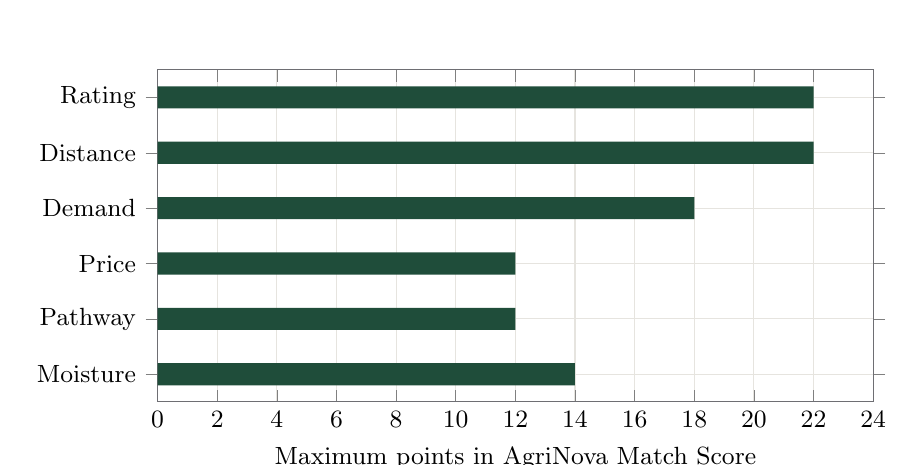
\begin{tikzpicture}
\begin{axis}[
  xbar,
  bar width=8pt,
  width=0.88\textwidth,
  height=5.8cm,
  xmin=0, xmax=24,
  xlabel={Maximum points in AgriNova Match Score},
  symbolic y coords={Moisture,Pathway,Price,Demand,Distance,Rating},
  ytick=data,
  tick label style={font=\small},
  xlabel style={font=\small},
  grid=major,
  major grid style={nvline},
  axis line style={nvmuted},
]
\addplot[fill=nvgreen, draw=none] coordinates {(14,Moisture) (12,Pathway) (12,Price) (18,Demand) (22,Distance) (22,Rating)};
\end{axis}
\end{tikzpicture}
\caption{Explainable match --- moisture can zero a lot that would otherwise look close.}
\label{fig:match}
\end{figure}

\section{Conclusions and impact of the activity}
This book farms \textbf{40.5 acres} (19.0 Madhyamgram--Barasat, 21.5 Punjab-by-phone). At 2.0~t/acre that is about \textbf{81~t} of straw. Last season \textbf{27~t was burned} (three Punjab calls) --- about Rs~19,000 at Rs~700/t, and about 40~tCO$_2$e as an estimate. Locally, five of six Bengal sheets never became a lot at all: they sat, dumped or mixed. Tapas's 1.5-acre heap at Hridaypur in September is the picture we started with: wet inside, too small to bale alone, still on the lane after rain.

Eight of ten said they would list in five days (\textbf{36 acres $\approx$ 72~t}, about \textbf{Rs~50,000} at the same gate). Tapas and Gurmeet are the Maybe lots --- too wet / too small --- which is why AgriNova needs a neighbourhood pool flag. The two ``sold'' rows are not a reason to stop: Anil still lost money on a moisture fight, and Balwinder still wants the spec on the slip before loading.

If those 72~t leave as a specified lot instead of smoke or mixed drain waste, the ward note can finally show utilised tonnes, and the farmer sees a gate price instead of a fine or a sweeper's complaint. That is the impact this activity can claim. It is a cluster demonstration on fourteen closed sheets, not a forecast for Punjab or North 24 Parganas.

Live desk: \url{https://agrinova-ochre.vercel.app}.

\begin{enumerate}
  \item From Dum Dum, the home failure is dump and mix. The phone-Punjab failure is burn. The shared cause is no plant number and no small-lot lift.
  \item Eight of ten will list if pickup is real. That is the opening.
  \item A conservancy pad will take a specified lot. It will not take mixed drain waste.
  \item Ward~21 Barasat and Madhyamgram SI will use an aggregate view. They will not put farmer phones on it.
  \item AgriNova is the listing between those two facts. Larger numbers on the website are demonstration examples, not this survey.
\end{enumerate}

No newspaper clipping is enclosed. Impact is 14 closed sheets, 72~t that would move, and a desk a judge can open.

\textbf{Limitations.} n=10, nearby plus phone. Civic names are public posts; comments are our notes of a student conversation, not a municipality circular. Carbon and Rs~700/t are working figures. September sittings recorded leftover already sitting locally, and last-season recall on the Punjab calls --- not a live October--November burn count.

\section{Suggested system or material for abatement}
AgriNova as a \textbf{ward / ULB listing} for Madhyamgram--Barasat, with a phone listing for the burn belt. The field test says the object is small: one card, one score, one trolley, one weekly total.

\begin{itemize}
  \item \textbf{Farm:} listing card --- acres, crop, tonnes (2.0~t/acre default), moisture, neighbourhood. Bangla voice here; Punjabi on the phone sheets.
  \item \textbf{Pad:} moisture on the slip. Reject mixed drain waste. Compost-first when the heap is wet (Hridaypur, Doltala); biomass-first when it is dry and baled (Kharar, Ghanaur).
  \item \textbf{Ward~21 / Madhyamgram SI:} weekly utilised vs dumped. No KCC, no Aadhaar, no farmer mobile.
  \item \textbf{Logistics:} one trolley serving listed lots in five days. Neighbourhood pool for 1.5--3 acre Maybe lots (Tapas, Gurmeet).
\end{itemize}

The abatement path, in order: (1)~farmer lists before the heap mixes or the window closes; (2)~score uses moisture so a wet lot is not sent to a $\le$15\% cabin; (3)~pickup date is visible; (4)~ward note records tonnes, not names. That is the system this book supports.

\subsection{Improvements suggested after field testing}
\begin{itemize}
  \item Wet / cannot-bale flag so Madhyamgram compost is offered before biomass.
  \item 1.5--3 acre lots auto-join a neighbourhood pool (Tapas at Hridaypur, Gurmeet at Rajpura rural).
  \item Conservancy complaint form: optional ``tonnes lifted this week'' --- still without names.
  \item SMS listing for keypad phones.
  \item Moisture written on the slip before the truck leaves the lane (Anil's Noapara condition).
\end{itemize}

\section{Acknowledgements}
We thank the six Madhyamgram and Barasat households who sat with us, and the four Punjab families who took a phone sheet. We thank Biswajit Ghosh (Madhyamgram conservancy pad) and Rakesh Kumar (Rajpura cabin, phone). We thank \textbf{Dr.\ Bibartan Saha}, Councillor, Ward No.~21, Barasat Municipality, and \textbf{Sudip Biswas}, Sanitary Inspector, Madhyamgram Municipality, for time on conservancy and mixed waste --- the views in this report are ours, not a ULB circular. We thank our science guide teacher at Kendriya Vidyalaya Dum Dum. Families helped with the Punjab calls. Errors remain ours.

\hfill Shikha Sharma \textbullet\ Samriddhi Ghosh \quad Class XI\\
\hfill Kendriya Vidyalaya Dum Dum, Kolkata

\section{References}
\begin{enumerate}[leftmargin=1.5em,itemsep=0.35em]
  \item Ministry of Environment, Forest and Climate Change. \textit{Solid Waste Management Rules, 2016}. Gazette of India, New Delhi, 2016. (Rules on biodegradable waste processing; see rr.\ 4--15.)
  \item Ministry of Agriculture \& Farmers Welfare. \textit{National Policy for Management of Crop Residue (NPMCR)}. New Delhi, 2014. pp.\ 1--12.
  \item Ministry of Agriculture \& Farmers Welfare. Crop Residue Management scheme guidelines (CRM / in-situ management). New Delhi, various years 2018--2024. Machinery and custom-hiring notes.
  \item Commission for Agricultural Costs and Prices. \textit{Price Policy for Kharif Crops: The Marketing Season 2024--25}. New Delhi, 2024. MSP table for common paddy (p.\ as notified).
  \item Indian Agricultural Research Institute / Punjab Agricultural University. Residue-to-grain ratio notes for rice (working band 1.8--2.4~t straw per acre). Bulletins and agronomy texts, various years.
  \item India Meteorological Department / IITM SAFAR. High-pollution episode briefs for Delhi--NCR, post-harvest months. PM$_{2.5}$ contribution discussion, various years.
  \item Central Pollution Control Board. Annual reports and residue-burning episode notes. New Delhi, selected years 2018--2024.
  \item IPCC. \textit{2006 IPCC Guidelines for National Greenhouse Gas Inventories}, Vol.~4, Agriculture, Forestry and Other Land Use. Chapter~2 / crop-residue burning factors. (2019 refinement used as order-of-magnitude only.)
  \item National Green Tribunal. Orders on crop-residue burning in NCR states (selected), 2015--2023.
  \item Government of Punjab. CRM / stubble-management public notes and biomass-procurement tender ranges (gate price band used as context). Chandigarh, recent seasons.
  \item West Bengal Pollution Control Board / municipal SWM processing notes. Mixed feedstock and compost-plant constraint (policy reading). Kolkata, recent years.
  \item United Nations. \textit{Transforming our world: the 2030 Agenda for Sustainable Development}. New York, 2015. SDG~2, 11, 12, 13 as theme alignment --- not as a data source.
  \item Barasat Municipality. Present Councillors (Ward No.~21: Dr.\ Bibartan Saha). \url{https://www.barasatmunicipality.org/present-councillors} (accessed 2026).
  \item Madhyamgram Municipality / SUDA (WB). Conservancy establishment --- Sanitary Inspector (Sudip Biswas) listing. Municipal / health nodal-officer notes.
\end{enumerate}

\end{document}
